\chapter{Introduction}


  The art of flock simulation has received increasing interests in the multi-media and entertainment industry. Bird flock scene is widely used in games and movies to make the scenes more rich or natural. However, since the number of objects involved is large, creating bird flock takes considerable time and efforts.


The work of Raynolds \cite{Boid, Steering} is our starting point about the study of a distributed behavior model. Reynolds proposed boid model, which described the behavior of large groups of birds, herds, and fish with perceptual skills existing in the real world. However, as stated by Reynold, the original boid model can only model flock wandering behavior. Controlling flock remains a necessary task for synthesizing bird flock. 


In this paper, we propose an alternative method for modeling bird flock. Our method uses a single RGB bird flock video as input to synthesize flock motion. The goal of our method is not to reproduce the exactly the same flock motion as it in the video. Instead, our method uses video as a reference to synthesize flocks that looks similar and natural to those in the video. We think perfect reconstruction of bird flock is nearly impossible without depth information, as we do not have precise three-dimension motion data as ground truth for evaluating our result.



The biggest challenge of this approach is that RGB video does not contain depth information. This makes flock motion synthesizing a difficult task. Human eyes can easily track moving objects, but tracking moving objects, especially bird flocks, is a challenging task in computer vision. The reason why we use RGB video as input is, obtaining depth information of bird flock with depth camera is difficult in outdoor scene. In work from Ju et al.\cite{Flappy}, or recording locomotion of a single bird as training data, they recorded the motion of dove using marker-based optical motion capture and high-speed video cameras for their work. They used 28 cameras to capture a single dove motion in region of 10m×10m×7m. Apparently, more space and devices are needed if we do the capture on a bird flock. In fact, we did capture bird flock motion by taking bird video using a 360-degree camera in outdoor scenes, but we failed to get useful video due to bad condition of outdoor environment. And it is also difficult to set up an indoor scene as they did for capturing bird flocks, since the space needed is too large. Thus, we consider predicting depth information of bird flock is helpful for making bird flock motion using real video as reference.


Two-dimensional projection data is the key information to predict three-dimension position. The main contribution of this research is to predict three-dimensional from two-dimensional tracking data retrieved from input video. That is, to predict distance from each bird to the camera in each frame. With predefined camera parameters, if we can predict the distance between the bird and the camera, three-dimensional position of the bird can be obtained.


Human eyes can easily track moving objects, but tracking moving objects, especially bird flocks, is a challenging task in computer vision. We use animal tracking technique for this task. This part is done using interactive feature tracking technique proposed by Buchanan et al.\cite{Tracking}. Interactive feature tracking is the process of extracting long and accurate tracks of three-dimensional features observed in two-dimensional video. Although the system is designed to track feature points, such as human face or eyes, it is also suitable for tracking bird flock, which contains multiple small trace targets that can also be treated as feature points.


\begin{figure}[h]
 \begin{center}
  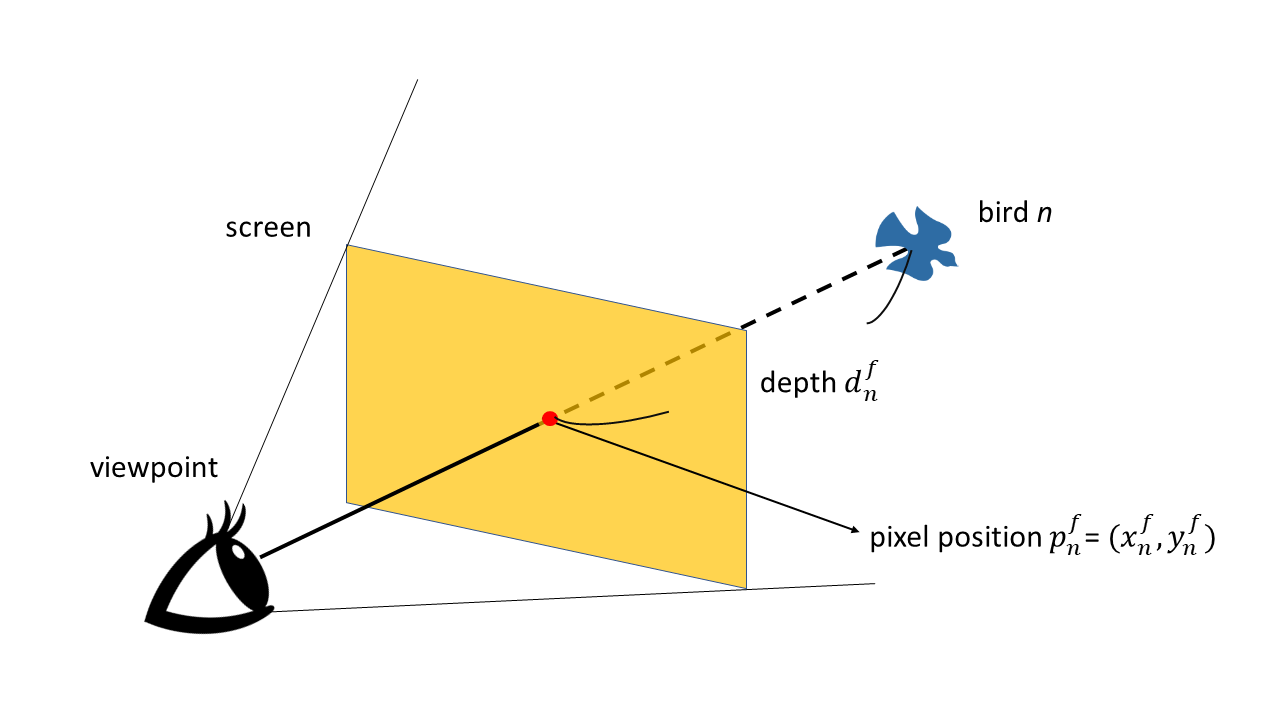
\includegraphics[width=1.0\textwidth]{view.eps}
 \end{center}
 \caption{View scenario}
 \label{figure:view}
\end{figure}


After the track data is obtained, predicting distance is next step. Based on our observations and boid flock models, we define two properties that a should have to retain the quality of flock motion. First, considering one bird flying trajectory, we do not expect a bird in frame $f$ to appear too far from its position in frame $f-1$ from its previous speed. That is, changes in position tend to be gradual. This is the first property: trajectory smoothness. Now we considering a group of birds. Reynolds proposed three steering behavior rules: separation, cohesion and alignment\cite{Boid}. In case of flock simulation, three rules are considered as three forces applied to each bird in each simulation steps. We also apply these rules in our system as the second property, flock behavior similarity. Considering these rules, target position in frame $f$ can be predicted if we have position in frame $f-1$. We consider an image sequence of length $F$ frames as input, with $N$ birds in each frame. Track data contains two-dimensional projection of each bird in the input video. The set of track data is denoted $P=\big\{p_n^f\big\}_{n=1...N,f=1...F}$ , where $p_n^f=(x_n^f, y_n^f)$, representing two-dimensional projection on screen, as shown in figure \ref{figure:view}. We want to predict depth $d_n^f$ of bird $n$ in frame $f$, while maintain the two properties above. The quality of a flight with a candidate depth set $X=\big\{d_n^f\big\}_{n=1...N,f=1...F}$ can be defined as:


\begin{equation}\label{eq:1}
 E(X) = \sum_{n = 1}^{N} \sum_{f = 1}^{F}e(n,f)
\end{equation}


\begin{equation}\label{eq:2}
 e(n,f) = \lambda_tt(p_n^f, p_n^{f-1},d_n^f) + \lambda_ff(p_n^f, p_n^{f-1},d_n^f)
\end{equation}


$e(n,f)$ denotes error function for bird n in frame f, which includes a trajectory smoothness term $t(.)$, and a flock behavior term $f(.)$. $\lambda_s$ and $\lambda_t$ are tuning parameters respecting to trajectory smoothness and flock behavior. Thus, the predicting problem can be restated as an optimization problem: choose $X$ to minimize $E(X)$. These terms will be further discussed in detail in later chapters.


Note that our contribution is in predicting three-dimensional flock motion from two-dimensional projection, not in tracking bird flocks.


The system presented in this paper can be separated into four stages. The first stage is trace retrieving stage. In this stage, trace data is retrieved by the system with user indications. Trace data contains projected two-dimensional positions in each frame for each bird. The system only allows user to retrieve trace for only one bird at a time, so trace data must be generated and saved for each bird before going to the next stage.


The second stage is optimization stage. In this stage, optimization is performed based on defined energy function to predict flock motion in three-dimensional space. Since the processing can be done in real time, user can adjust parameters to the systems and see the result directly for better results.


The last stage is refinement stage. Since the system only predict the position in last stage, the orientation of each bird is calculated based on its position in each frame to complete the flock motion as output.


We implemented a flock simulation system to synthesize bird videos that fit the requirements of the system. Despite we used generated results as inputs, we assume the 2D projection to the camera is unknown. This assumption makes the system can also be used for real bird video.


The structure of the paper is as follows: In chapter 2, we discuss related work. In chapter 3, we present the overall design of our system discussing the requirements needed for predicting flock motion. In chapter 4, we present the results generated by our system. In chapter 5, we discuss about future work and limitations of our system. Finally, we summarize this research in chapter 6.

